\chapter{Exercise 02}
%******************************************************************************%
%                                                                              %
%                                 Interlude                                    %
%                         for Machine Learning module                          %
%                                                                              %
%******************************************************************************%

\section*{Interlude - Predict, Evaluate, Improve}

\epigraph
{A computer program is said to learn from experience E, with respect to some
class of tasks T, and performance measure P, if its performance at tasks in T,
as measured by P, improves with experience E.}{\textit{Tom Mitchell,\\Machine Learning, 1997}}

\begin{quote}{}

\end{quote}

In other words to learn you have to improve.\\
To improve you have to evaluate your performance.\\
To evaluate your performance you need to start performing on the task you want to be good at.


One of the most common tasks in Machine Learning is \textbf{prediction}.\\  
This will be your algorithm's task.\\
This will be your task.  

\begin{figure}[h!]
  \centering
  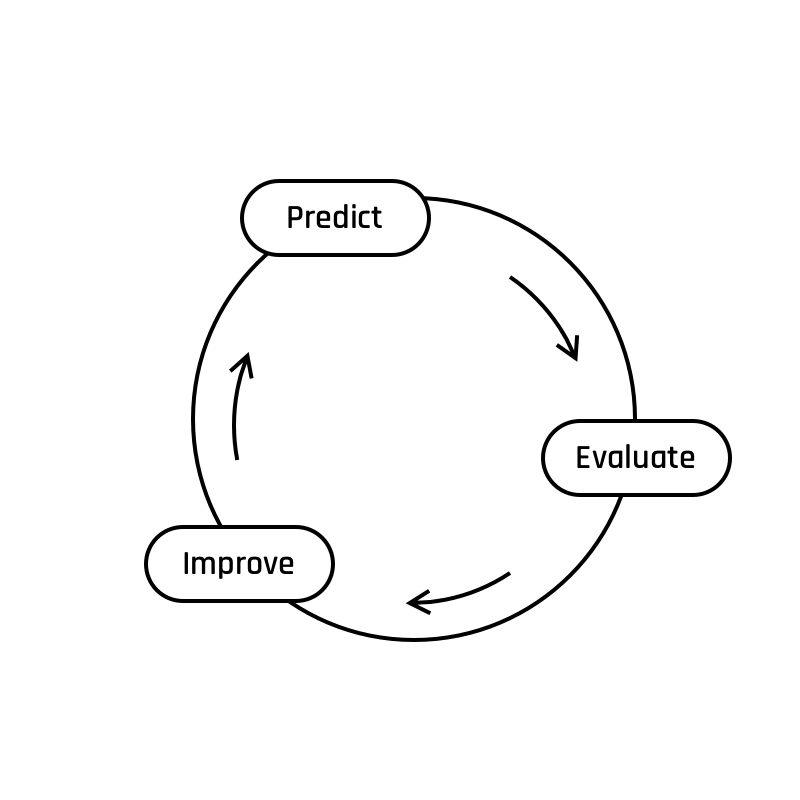
\includegraphics[scale=0.25]{assets/Default.png}
  \caption{cycle neutral}
\end{figure}

\section*{Predict}

\begin{figure}[h!]
  \centering
  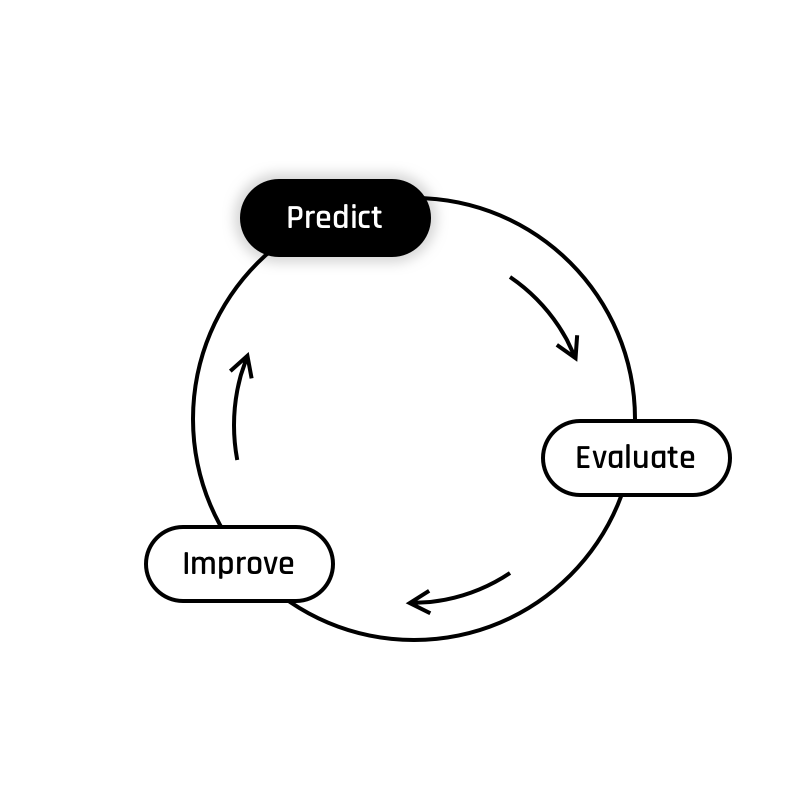
\includegraphics[scale=0.25]{assets/Predict.png}
  \caption{cycle predict}
\end{figure}

\subsection*{A very simple model}

We have some data. We want to model it.  
\begin{itemize}
    \item First we need to \textit{make an assumption}, or hypothesis, \textit{about the structure of the data and the relationship between the variables}.  
    \item Then we can \textit{apply that hypothesis to our data to make predictions}.
\end{itemize}

$$
hypothesis(data) = predictions
$$

\subsubsection*{Hypothesis}
Let's start with a very simple and intuitive \textbf{hypothesis} on how the price of a spaceship can be predicted based on the power of its engines.\\
We will consider that \textit{the more powerful the engines are, the more expensive the spaceship is}.\\
Furthermore, we will assume that the price increase is \textbf{proportional} to the power increase. In other words, we will look for a \textbf{linear relationship} between the two variables.

This means that we will formulate the price prediction with a \textbf{linear equation}, that you might be already familiar with:

$$
\hat{y} = ax + b
$$

We add the \texttt{\^} symbol over the $y$ to specify that $\hat{y}$ \textit{(pronounced y-hat)} is a \textbf{prediction} (or estimation) of the real value of $y$. The prediction is calculated with the \textbf{parameters} $a$ and $b$ and the input value $x$.

For example, if $a = 5$ and $b = 33$, then $\hat{y} = 5x + 33$.

But in Machine Learning, we don't like using the letters $a$ and $b$. Instead we will use the following notation:

$$
\hat{y} = \theta_0 + \theta_1 x
$$

So if $\theta_0 = 33$ and $\theta_1 = 5$, then $\hat{y} = 33+ 5x$.

To recap, this linear equation is our \textbf{hypothesis}. Then, all we will need to do is find the right values for our parameters $\theta_0$ and $\theta_1$ and we will get a fully-functional prediction \textbf{model}.


\subsubsection*{Predictions}
Now, how can we generate a set of predictions on an entire dataset? Let's consider a dataset containing $m$ data points (or space ships), called \textbf{examples}.

What we do is stack the $x$ and $\hat{y}$ values of all examples in vectors of length $m$. The relation between the elements in our vectors can then be represented with the following formula:

$$
\begin{matrix}
\hat{y}^{(i)} = \theta_0 + \theta_1 x^{(i)} & & \text{ for i = 1, ..., m}
\end{matrix}
$$  

Where:
\begin{itemize}
    \item $\hat{y}^{(i)}$ is the $i^{th}$ component of vector $y$
    \item $x^{(i)}$ is the $i^{th}$ component of vector $x$   
\end{itemize}

Which can be experessed as:

$$
\hat{y} = \begin{bmatrix}\theta_0 + \theta_1 \times x^{(1)} \\ \vdots \\  \theta_0 + \theta_1 \times x^{(m)}\ \end{bmatrix}
$$  

For example,

$$
\text{given } \theta = \begin{bmatrix}33 \\ 5 \end{bmatrix} \text{ and } x = \begin{bmatrix}1 \\ 3 \end{bmatrix} \text{: }
$$

$$
\hat{y} = h_{\theta}(x) = \begin{bmatrix} 33 +  5 \times 1 \\ 33 + 5 \times 3\end{bmatrix}  = \begin{bmatrix} 38 \\ 48 \end{bmatrix} 
$$

\newpage

\subsection*{More information}

\subsubsection*{Why the $\theta$ notation?}

You might have two questions at the moment:
\begin{itemize}
    \item \textbf{WTF is that weird  symbol?}
    This strange symbol, $\theta$, is called "theta".
    
    \item \textbf{Why use this notation instead of $a$ and $b$, like we're used to?}
    Despite its seeming more complicated at first, the theta notation is actually meant to simplify your equations later on. Why?
    $a$ and $b$ are good for a model with two parameters, but you will soon need to build more complex models that take into account more variables than just $x$.
    You could add more letters like this:  $\hat{y} = ax_1 + bx_2 + cx_3 + ... + yx_{25} + z$  
    But how do you go beyond 26 parameters? And how easily can you tell what parameter is associated with, let's say, $x_{19}$? That's why it becomes more handy to describe all your parameters using the theta notation and indices.
    With $\theta$, you just have to increment the number to name the parameter:
    $\hat{y} = \theta_0 + \theta_1 x_1 + \theta_2 x_2 + ... + \theta_{2468} x_{2468}$ ... Easy right?
\end{itemize}


\subsubsection*{Another common notation}

$$
\begin{matrix} & & \hat{y} & = & h_{\theta}(x)\end{matrix}
$$

Because $\hat{y}$ is calculated with our linear hypothesis using $\theta$ and $x$, it is sometimes written as $h_{\theta}(x)$.
The $h$ stands for \textit{hypothesis}, and can be read as \textit{"the result of our hypothesis h given x and theta"}.

Then if $x = 7$, we can calculate:
$\hat{y} = h_{\theta}(x) = 33 + 5 \times 7 = 68$
We can now say that according to our linear model, the \textbf{predicted value} of $y$ given ($x = 7$) is 68.

\newpage
\extitle{Logistic Loss Function}
\turnindir{ex02}
\exnumber{02}
\exfiles{log\_loss.py}
\exforbidden{None}
\makeheaderfilesforbidden

% ================================= %
\section*{Objective}
% --------------------------------- %
Understanding and manipulation of the loss function in the context of logistic regression.\\
\\
You must implement the following formula as a function:  

$$
J( \theta) = -\cfrac{1} {m} \lbrack \sum_{i = 1}^{m} y^{(i)}\log(\hat{y}^{(i)})) + (1 - y^{(i)})\log(1 - \hat{y}^{(i)})\rbrack
$$
Where:
\begin{itemize}
  \item $\hat{y}$ is a vector of dimension $m$, the vector of predicted values
  \item $\hat{y}^{(i)}$ is the $i^{th}$ component of the $\hat{y}$ vector
  \item $y$ is a vector of dimension $m$, the vector of expected values
  \item $y^{(i)}$ is the $i^{th}$ component of the $y$ vector
\end{itemize}

% ================================= %
\section*{Instructions}
% --------------------------------- %
In the \texttt{log\_loss.py} file, write the following function as per the instructions below:
\\
\par
\begin{minted}[bgcolor=darcula-back,formatcom=\color{lightgrey},fontsize=\scriptsize]{python}
def log_loss_(y, y_hat, eps=1e-15):
    """
    Computes the logistic loss value.
    Args:
        y: has to be an numpy.ndarray, a vector of shape m * 1.
        y_hat: has to be an numpy.ndarray, a vector of shape m * 1.
        eps: has to be a float, epsilon (default=1e-15)
    Returns:
        The logistic loss value as a float.
        None on any error.
    Raises:
        This function should not raise any Exception.
    """
    ... Your code ...
\end{minted}

\hint{
  The logarithmic function isn't defined in $0$.
  This means that if $y^{(i)} = 0$ you will get an error when you try to compute $log(y^{(i)})$.
  The purpose of the \texttt{eps} argument is to avoid $log(0)$ errors.
  It is a very small residual value we add to \texttt{y}, also referred to as `epsilon`.
}

% ================================= %
\section*{Examples}
% --------------------------------- %
\begin{minted}[bgcolor=darcula-back,formatcom=\color{lightgrey},fontsize=\scriptsize]{python}
# Example 1:
y1 = np.array([1]).reshape((-1, 1))
x1 = np.array([4]).reshape((-1, 1))
theta1 = np.array([[2], [0.5]])
y_hat1 = logistic_predict_(x1, theta1)
log_loss_(y1, y_hat1)
# Output:
0.01814992791780973

# Example 2:
y2 = np.array([[1], [0], [1], [0], [1]])
x2 = np.array([[4], [7.16], [3.2], [9.37], [0.56]])
theta2 = np.array([[2], [0.5]])
y_hat2 = logistic_predict_(x2, theta2)
log_loss_(y2, y_hat2)
# Output:
2.4825011602474483

# Example 3:
y3 = np.array([[0], [1], [1]])
x3 = np.array([[0, 2, 3, 4], [2, 4, 5, 5], [1, 3, 2, 7]])
theta3 = np.array([[-2.4], [-1.5], [0.3], [-1.4], [0.7]])
y_hat3 = logistic_predict_(x3, theta3)
log_loss_(y3, y_hat3)
# Output:
2.9938533108607053
\end{minted}

\info{
  This function is called \textbf{Cross-Entropy loss}, or \textbf{logistic loss}.
  For more information you can look at \href{https://en.wikipedia.org/wiki/Cross_entropy\#Cross-entropy\_error\_function\_and\_logistic\_regression}{this section}
  of the Cross entropy Wikipedia article.
}